\section{Configuration}

% TODO Define configuration and which constructs we want to be configurable

\subsection{Motivation}

From observation 2 we saw that most configuration was done via the inclusion of
source code. This source code would expose constants (read: literal values
\emph{and} identifiers). The included source code, however, can do anything
that Jolie source normally can, and isn't limited to just the desired
configuration. As a result, a service developer cannot be certain that the
configurator (entity who provides configuration) doesn't start messing with
other details of the program. Deploying defensive
programming\footnote{Defensive programming techniques are usually employed for
systems that require high availability, or where safety and security is
required.} techniques against this becomes significantly more problematic,
since no guarantees about the configuration source file can really be made.

Distributing re-useable packages is also problematic with this approach.
Several features of package management requires that the package remains
read-only. For example, updating of packages require this, without it
source-code merges would be required.

We also saw that a lot of issues, that should have been a deployment issue,
became a code issue.

This gives us plenty of reason to explore the need for a native configuration
format.  Most other systems would most likely go for a system defined in user
code, as opposed to natively. An example of such framework, could be Vert.x, it
is a tool-kit for building reactive applications on the JVM.  Examples of such
``reactive applications'' are microservices. The configuration workflow is
shown in Figure \ref{fig:normal_conf}. The system will retrieve, and read
external configuration files, directed by the user code, and apply the
configuration as needed.

% Most other systems can do this at run time
% For example Vert.x does this by reading external configuration files
% Once configuration is done, we can start up the server

\begin{listing}[H]
\begin{minted}{text}
+------------------+     +-------------------+     +--------------------+
| executable start | --> | retrieve conf     | --> | read conf files    |
+------------------+     +-------------------+     +--------------------+
                                                             |
                            +-----+                          |
                            |     | reconfigure              |
                            |     v                          v
                         +-------------------+     +--------------------+
                         | server running    | <-- | perform conf       |
                         +-------------------+     +--------------------+
\end{minted}
\caption{Simplified workflow for configuration of Vert.x applications}
\label{fig:normal_conf}
\end{listing}

% http://vertx.io/blog/vert-x-application-configuration/
% http://vertx.io/docs/vertx-config/kotlin/

TODO Defined deployment time somewhere

However implementing such as a system in Jolie has its problems, most of these
come from the difference between general-purpose programming languages and
specialized programming languages.

In general-purpose languages, the constructs (such as a server's socket) for
the microservice architecture are created in user code. As a result they are
entirely accessible from user code. This make it feasible to change their
behaviour, since code can run before deployment occurs.

In Jolie the constructs are managed directly by Jolie. Doing this has multiple
advantages, such as less complexity in user code, but it also means that user
code is capable of doing less. Jolie user code can for example not control
networking directly, but is instead forced to use the abstractions provided by
Jolie (sending messages). The language puts constraints on certain
constructs being fully prepared directly in the source code. This is analogous
to a programming language requiring the types of a struct's field to be present
at compile time. As a result, not all constructs can be changed at run time.
Concrete examples of this includes the input ports, which needs to be ready at
deployment time. Thus without native support for configuration of these, it
would not be possible to change the input port.

\subsection{Configuration Units}
\label{sec:conf_units}

A configuration unit is the basic entity, which encapsulates the configuration
of a single Jolie module. A configuration unit is known by its name (known as
its ``profile''), along with which module it configures. Having multiple profiles
for the same module can be useful for a variety of use-cases. A common
use-case, could for example be to have separate profiles for development and
production.

The units hold configuration for every possible type of configurable construct
in Jolie. The ones supported are:

\begin{enumerate}
    \item Input and output ports
        \begin{itemize}
            \item Location
            \item Protocol and protocol parameters
            \item Embedding of other services (output ports only)
        \end{itemize}
    \item General purpose parameters
    \item Interface rebinding
\end{enumerate}

In the coming sections we'll mostly focus on the first two, in Section
\ref{sec:interface_rebinding} we'll cover interface rebinding.

% TODO Do we allow for inclusion of other files?
Configuration units are defined in configuration files, which may contain
several units. These files may even include other files, to pull in more
configuration units.

Jolie provides a new configuration file format. This format is custom, and made
to mimic the syntax of Jolie. Listing \ref{lst:simple_conf} shows a very
simple configuration unit. This units sets the location and protocol for the
output port \mintinline{jolie}{A}, the location of the input port
\mintinline{jolie}{ModuleInput}, and a parameter.

\begin{listing}[H]
\begin{minted}{jolie}
profile "hello-world" configures "my-module" {
    outputPort A {
        Location: "socket://a.example.com:3000"
        Protocol: sodep { .keepAlive = true }
    },

    inputPort ModuleInput {
        Location: "socket://localhost:80"
    },

    myParameter = 42,
    myParameter.subProperty = "hello"
}
\end{minted}

\caption{A simple configuration unit named \mintinline{jolie}{hello-world}
    configuring the module \mintinline{jolie}{my-module}}

\label{lst:simple_conf}

\end{listing}

Embedding of output ports can be performed from within a configuration unit.
This moves the embedding from being a code problem to, what it should have
been, a deployment problem. Listing \ref{lst:conf_embedding} shows the
embedding of output port \mintinline{jolie}{A}. Note that we need to make a
reference to the module, since the profile names are placed under a namespace
for each module. This way multiple services can share the same name, a
situation which is likely to occur with common profile names, such as
``development'' and ``production''.

\begin{listing}[H]
\begin{minted}{jolie}
profile "hello-world" configures "my-module" {
    outputPort A embeds "a-module" with "a-profile"
}

profile "a-profile" configures "a-module" {
    // configuration of a-module goes here.
}
\end{minted}
\caption{Embeddings make reference to other configuration units}
\label{lst:conf_embedding}
\end{listing}

As we can see from the examples, it is not necessary to provide all the values
of a port. It isn't necessary for two reasons. The first reason is that certain
values may be provided by the underlying module, which uses this unit. If a
module provides a value, then the configuration unit cannot override it. The
second reason is that configuration profiles may extend other profiles.

Configuration units may extend another unit, which configures the same module.
The tree of inheritance may be of an arbitrary depth, but each unit may only
extend a single unit, and they must configure the same module. The child is
also wins when it comes to configuration. This means that if unit ``B'' extends
``A'', and they both configure the same value, then the values found in B is
the one that is correct. Listing \ref{lst:conf_extends} shows an example of
extension with units.

\begin{listing}[H]
\begin{minted}{jolie}
profile "a" configures "a-module" {
    aValue = 42,
    aValue.sub = "hello",

    outputPort ExternalService {
        Location: "socket://external.example.com:42000"
    }
}

profile "b" configures "a-module" extends "a" {
    aValue = 100
    // aValue.sub = "hello"
    // ExternalService.location = "socket://external.example.com:42000"
}
\end{minted}
\caption{Configuration units may extend other units}
\label{lst:conf_extends}
\end{listing}

The module developer is often aware of what the defaults should be. For this
reason default configuration profiles may be shipped along the modules, which
are implicitly imported into every configuration file. The Jolie engine will
look for any \mintinline{text}{.col} file\footnote{The file extension of the
configuration file} in the \mintinline{text}{conf} folder. This folder
should be placed relative to the module's root. For example, if module "a" has
a file called \mintinline{text}{conf/my-defaults.col}, which contains a unit
called "default". Then the user of the package may either write a configuration
unit which extends this, simply by writing \mintinline{jolie}{profile
"something" configures "a" extends "default"}, or the default
directly. There is no need for any inclusion of this file.

It should be noted that no single unit is required to provide all
configuration. The system doesn't have any ``abstract''\footnote{As in abstract
classes, a concept often used in object oriented programming} configuration
units. However it is required that the configuration file provides all the
necessary configuration, as declared by the module. We'll learn more about
how a module declares configuration in Section \ref{sec:ol_conf}.

\subsection{Configuration and the Core Language}
\label{sec:ol_conf}

In section \ref{sec:conf_units} we learned about the configuration files, but
never actually saw the corresponding Jolie modules. In this section we'll
discover how the language has changed to accommodate this configuration
feature.

The configuration system provides the ability to configure any type of port,
and additional provide the module with ``parameters''. Ports were covered in
section TODO. Most importantly it should be noted that output ports do not
require any values at deployment time, and can be changed at run time, while
input ports require all their values at deployment time, and cannot be changed
at run time. % TODO Do we want to cover why it is hard to change input ports at
% run time?

\begin{listing}[H]
\begin{multicols}{2}
\begin{minted}[breaklines,fontsize=\footnotesize]{jolie}
outputPort Service {
    Location: "socket://service.example.com:443"
    Protocol: https {
        .debug = true,
        .debug.showContent = false
    }
    Interfaces: IService
}
\end{minted}

\columnbreak

\begin{minted}[breaklines,fontsize=\footnotesize]{jolie}
outputPort Service {
    Interfaces: IService
}
\end{minted}

\end{multicols}

\caption{
    Two valid output ports.
    (Left) A fully configured output port.
    (Right) A minimal output port.
}

\label{lst:basic_output}
\end{listing}

Listing \ref{lst:basic_output} shows a two different output ports, both
perfectly valid.

TODO

When should we configure? Go through a few different approaches, always
override source, always let code win, do we let everything be configurable?
Should configuration stay final, or should we allow changing it later?  How do
we distinguish between accidentally leaving something out and wanting it to be
configurable?

Output ports

Input ports, and why they are harder.

The \mintinline{jolie}{dynamic} keyword has been introduced to deal with which
ports that should allow configuration, any port which does not have the dynamic
keyword is static. Only ports which are static should be configurable. TODO Why
is this a good idea.

Parameters

\subsection{Implementing the Configuration Format}

Implementation, and fixing the AST

\subsection{Example}

TODO This is just copy pasted from some markdown document. Might be able to
find a better example. Syntax is most likely also outdated.

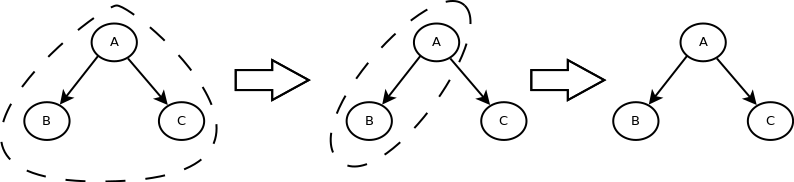
\includegraphics[width=\textwidth]{prototypes.png}

(The dashed region corresponds to which services that are embedded together)

This use-case is intended to show how we can easily go from a prototype where
we embed everything (this is easier to run locally) to hosting each service by
itself.

\begin{minted}{jolie}
// A.ol

ext outputPort A {
    Interfaces: AIface
}

ext outputPutPort B {
    Interfaces: BIface
}

constants {
    FOO: int
}
\end{minted}

\begin{minted}{jolie}
// A.col

include "B.col" // The includes work just like they do in Jolie
include "C.col"

// Previously called namespace. Configures makes it more explicit that we're
// talking about a specific package and not an arbitrary name
configures "A" {
    // Like always we just put the definitions here
    FOO = 42

    // We alter the syntax slightly for output ports being embedded
    outputPort B embeds B
    // The second B refers to the profile B (if no profile is specified it gets
    // the same name as the package it configures). This means that this
    // configures block also has name "A". It could also have been written as:
    // `profile "A" configures "A"`

    outputPort C embeds C
}
\end{minted}

Note: The previous proposal did not allow for embedding of services directly
from the configuration. This is however needed since packages by themselves
should be considered read-only. Thus if we want to configure a package to embed
its dependencies, then this must be done from external configuration, we cannot
do this in source.

\begin{minted}{jolie}
// B.col

configures "B" {
    inputPort B {
        Location: "local"
    }
}
\end{minted}

\begin{minted}{jolie}
// C.col

configures "C" {
    inputPort C {
        Location: "local"
    }
}
\end{minted}

In order to use an external B we need to update "A.col":

\begin{minted}{jolie}
// A.col
include "C.col"

configures "A" {
    outputPort B {
        Location: "socket://b.example.org:8000"
        Protocol: sodep
    }
    outputPort C embeds C
}
\end{minted}

In order to update the deployment file of B we simply need to update the
input port to no longer be local.

\begin{minted}{jolie}
// B.col
configures "B" {
    inputPort B {
        Location: "socket://localhost:8000"
        Protocol: sodep
    }
}
\end{minted}

In most cases however this would be unnecessary since the default
configuration file for "B" could already include a default input port.

In that case we could simply deploy directly from the default configuration.
The restriction on configuration units to only configure a single package helps
a lot. This restriction means that we cannot from any node configure any other
node which isn't a direct child of it. Without this we wouldn't be able to
easily swap out one configuration unit for another.

